\section{Predicting cell organelles}
\subsection{Loss}
Although one can easily define a loss function like MSE or Pearson correlation coefficient between ground truth and predicted fluorescence image, there is still a problem is relating this metric to estimating quality of predicted images in practice. There is a clear need to clearly state the down-stream tasks that are going to be performed in the predictions from our data. However these downstream tasks might be different and are not determined right away. For example even though the training of the model happens with the use of Pearson score or MSE, the real practical evaluation will happen in terms of metrics like: the number of the nuclei in the image, the closeness of the intensities of the nuclei of interest, the difference in their mean intensities, the level of details in the Golgi apparatus and the strength of the non specific background fluorescence noise. These metrics are not known in advance and therefore there will always be a gap between the metrics that are used during train and the metrics that are used in practice.

During training 2 following losses have beed used. MSE loss:

\begin{equation}
    Loss_{MSE} = \frac{1}{N} \sum_{i=1}^{N}{\sum_{j=1}^{W}{\sum_{k=1}^{H}{(y_{j,k} - \hat{y}_{j,k})^2}}}
\end{equation}

where $N$ is the number of images in the batch and $y_{j,k}$ and $\hat{y}_{j,k}$ are the \{j,k\}th pixel of the ground truth and predicted images respectively.

Pearson Correlation Coefficient (PCC) is commonly used in cell biology when comparing the co-localization of two or more proteins, and also used in computer vision to assess spatial-intensity when determining image similarity (reword and cite Cohen). It is calculated as follows:

\begin{equation}
    Loss_{PCC} = \frac{\sum_{i=1}^{N}{(y_i - \bar{y_i})(\hat{y_i} - \bar{\hat{y_i}})}}{\sqrt{\sum_{i=1}^{N}{(y_i - \bar{y_i})^2(\hat{y_i} - \bar{\hat{y_i}})^2}}}
\end{equation}

where $y_i$ is the flattened ground truth image, $\hat{y_i}$ is flattened predicted image and $\bar{y_i}$, $\bar{\hat{y_i}}$ are means of the ground truth and predicted images respectively.

\subsection{Nuclei}
In this subsection the results of the nuclei predictions will be presented. You can see examples of predictions presented in Figures TODO and TODO. There are TODO visible problems with the predictions:
\begin{itemize}
    \item The form of the nucleus is captured, but the texture inside is not
    \item Blurry border aorund the nuclei
    \item Problems with the predictions on the borders of the crop
\end{itemize}
Predictions of the border of the crops are quite challenging for the model as there is not enough of the information due to the cropped parts of the cell. However this can be easily solved with using overlaps while cropping the image to avoid the use of the pixels predicted on the border. There more information on this in Chapter TODO (Crops combination).

Explanation for the lack of details inside TODO

The nucleus is relatively a simple task for predictions as it might be relatively easier to spot the nuclei manually as well. They are relatively big with respect to the cell as well. More challenging task would be a prediction of Golgi Apparatus.

\subsection{Golgi Apparatus}
Golgi Apparatus (or simply Golgi) is another organelle inside the cell, that packages protein into membrane-bound vescicles. One can see an example of how the staining of the Golgi with fluorescence imaging looks like in Figure TODO ref. It is evident that there is a lighter foreground fluorescence and a bit darker one apart from the black background itself. Truly Golgi is only the lighter part of fluorescence lightning and the other part is called a non-specific fluorescence lightning. It comes from the cell itself, and might occur when the antigen is impure and contains antigenic contaminants. (cite Immunofluorescence in medical science indian) Its brightness may vary due to longer or shorter exposure time. 

Having such a non-specific fluorescence background may have 2 potential challenges for training:
\begin{itemize}
    \item The relative area of the background fluorescence is bigger than the area of Golgi themselves. Therefore quite a big part in the loss during training will be dedicated to teaching model to restore this background fluorescence instead of the Golgi itself.
    \item It also introduces difficulties during the post-processing of the predictions. As well as for nuclei, the mask of the predicted Golgi Apparatuses will be needed. Using the same algorithm for post-processing segmentation that was used for nuclei, the mask of the Golgi Apparatus will consider the background noise to be relevant, although this is an unwanted behavior.
\end{itemize}

To escape this one has to subsctract the background first or so-called to enhance the image. The main approach was to replicate the post-processing that is used in practice in labs for segmenting fluorescence images of Golgi.

\begin{figure}[htb]
	\begin{center}
		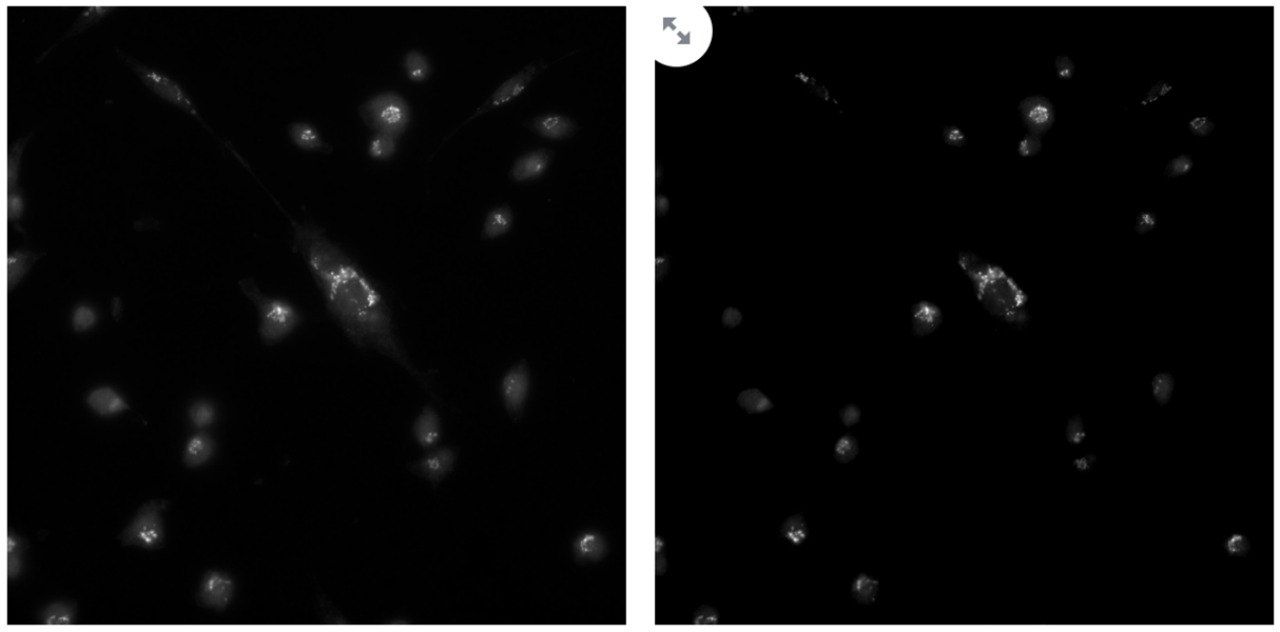
\includegraphics[width=0.5\linewidth]{bilder/enhancement.jpg}
		\caption{Golgi enhancement}\label{fig:golgi-enhancement}
	\end{center}
\end{figure}

On the left of Figure \ref{fig:golgi-enhancement} one can see the original ground truth image and on the right - the images after the background was substracted. To do so the rolling ball algorithm has been used.

\subsubsection{Rolling ball algorithm}
Rolling ball algorithm has been introduced by Sternberg in 1983 (cite doi:10.1109/mc.1983.1654163) and is still widely used for processing medical and biological data. The idea of this algorithm is based on morphological opening of the image. 

Morphological opening is an operation on the image involving first eroding the image and then dilating it with the same structuring element for both operations. It is helpful for extracting big image features. (cite https://cutt.ly/PGJjucI) Structuring element is a matrix smaller than the image itself that defines the area around the pixel that is going to be processed to define its new value after the morphological operation is performed. It is an analogues of a kernel in image processing. You can see an example of a structuring element on the Figure \ref{fig:structuring-element}

\begin{figure}[htb]
	\begin{center}
		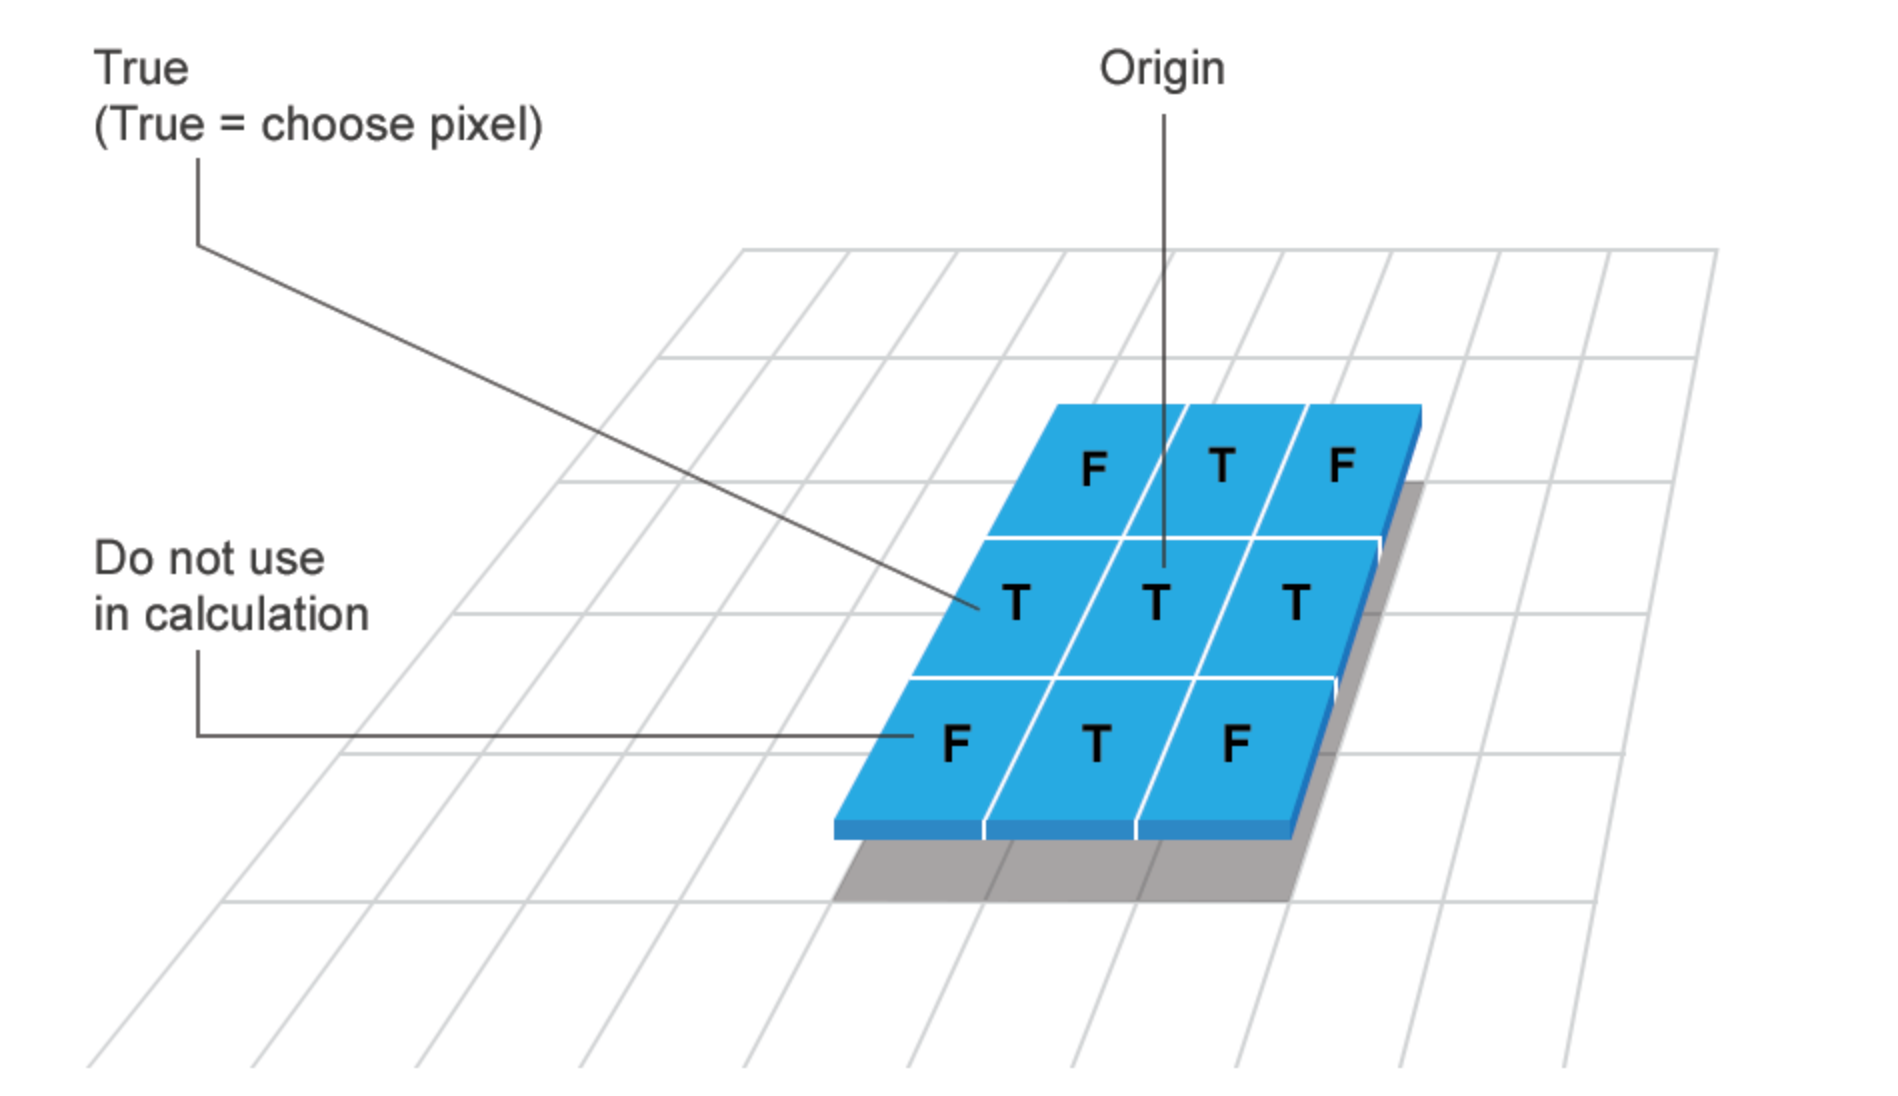
\includegraphics[width=0.5\linewidth]{bilder/structuring-element.png}
		\caption{Structuring Element}\label{fig:structuring-element}
	\end{center}
\end{figure}

Morphological dilation takes a new value of the pixel as the maximum value of its neighbours within the structing element. Therefore after this operation lines will be thicker and in general objects will appear bigger.

Morphological erosion on the other hand makes the pixel value as the minimum value of its neighbours within the structuring element. After this operation the floating pixels will be removed and all object become smaller and thinner.

Sternberg has extrapolated the operation of morphological opening from 2D into 3D space. If one can imagine the image to be a 3D plane, with the height of ech pixel being determined by its intesity, such an interpretaion of the image is called umbra. The structuring element for morphological opening of an umbra has to be then also a 3D object - a ball for example. The opening of an umbra then will be a union of translations of the 3-D structuring element that can be rntirely contained inside umbra (see Figure \ref{fig:rolling-ball}). One can image the ball freely moving inside the volume constrained by the upper surface of an umbra. The opening then consists of all the pixels then can be reaches by the ball. The radius of the ball then is the hyper-parameter than has to be tuned. 

\begin{figure}[htb]
	\begin{center}
		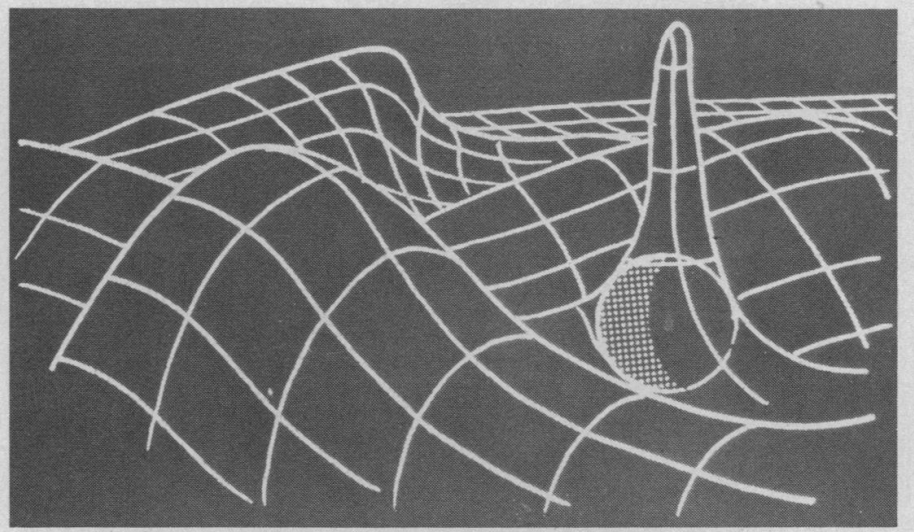
\includegraphics[width=0.5\linewidth]{bilder/rolling-ball.png}
		\caption{Rolling Ball}\label{fig:rolling-ball}
	\end{center}
\end{figure}

However, subtracting the background with rolling ball algorithm is not enough to get a reasonably clean signal of Golgi Apparatus from fluorescence imaging. To check this one can convert the original image from the vanilla pre-processing with rolling ball algorithm into a mask. To do so, let's just assing all non-zero pixels to the maximum value of image intensity. The mask that have been created like this would look like in Figure \ref{subfig:vanilla-mask}. It clearly still contains a lot of background noise of low intensity and that is why this background noise was not visible for an eye. In order to remove it one could clip lower intensities of the image via the following approach:

\begin{lstlisting}
	import numpy as np
		
	def clip(image):
		minval = np.percentile(image, 90)
		image = np.clip(image, minval, image.max())
		image = (image - image.min()) / (image.max() - image.min())
		return image
\end{lstlisting}


\begin{figure}
	\centering
	\begin{subfigure}[b]{0.22\textwidth}
		\centering
		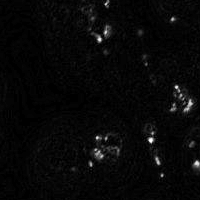
\includegraphics[width=\textwidth]{bilder/preprocessing/crop_golgi_not_full_processed.png}
		\caption{}
		\label{subfig:vanilla}
	\end{subfigure}
	\hfill
	\begin{subfigure}[b]{0.22\textwidth}
		\centering
		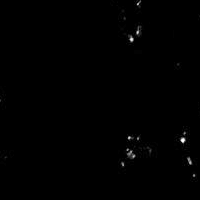
\includegraphics[width=\textwidth]{bilder/preprocessing/crop_golgi_full_processed.png}
		\caption{}
		\label{subfig:clipping}
	\end{subfigure}
	\hfill
	\begin{subfigure}[b]{0.22\textwidth}
		\centering
		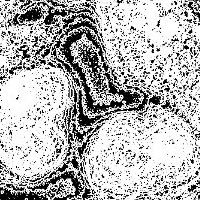
\includegraphics[width=\textwidth]{bilder/preprocessing/crop_golgi_not_full_processed_mask.png}
		\caption{}
		\label{subfig:vanilla-mask}
	\end{subfigure}
	\hfill
	\begin{subfigure}[b]{0.22\textwidth}
		\centering
		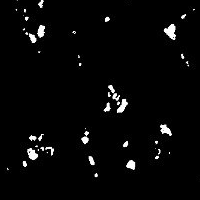
\includegraphics[width=\textwidth]{bilder/preprocessing/crop_golgi_full_processed_mask.png}
		\caption{}
		\label{subfig:clipping-mask}
	\end{subfigure}
	   \caption{(a) Vanilla pre-processing with automatic background removal algorithm only; (b) Additional clipping of lower intensities after vanilla pre-processing; (c) masked or subfigure (a); (d) mask of subfigure (b)}
	   \label{fig:pre-processing-golgi}
\end{figure}

The result of the clipped image and its mask are illustated in the Figure \ref{subfig:clipping}, \ref{subfig:clipping-mask} correspondingly. It contains almost no background noise now. Such additional clipping might improve the results slightly.